\documentclass[../main.tex]{subfiles}
\usepackage[utf8x]{inputenc}
\usepackage{blindtext}
\usepackage{float}
\usepackage{graphicx}
\usepackage{siunitx}
\usepackage{cite}

\begin{document}

As it's been noted, malware can be something as simple as ads to something as complex as kernel rootkits. While anti-virus software does exist, it exists within a cycle with malware. As new anti-virus software is released, malware is created to combat it and this cycle goes on and on and on. This continuation of the cycle has led to the research and development of hardware-based malware detection techniques on the very basis of software-based defenses being easier to bypass \cite{theoretical}. One method to the hardware-based malware detection issue is, using HPCs. Since HPCs periodically monitor HPC readings and compare those very readings to a "golden" HPC reading, they then report the inconsistencies \cite{theoretical}. 

Since HPC-based profilers are nearly ubiquitous, the very first instance of using HPCs as a trusted mode of detecting malware was for the use of program integrity checks. In this experiment, malicious program changes were monitored at two different phases: statically during the load phase and then dynamically at runtime.

HPCs typically operate in two phases: offline and online, the figure below, taken from \cite{theoretical}, shows that:

\begin{figure}[h]
    \centering
    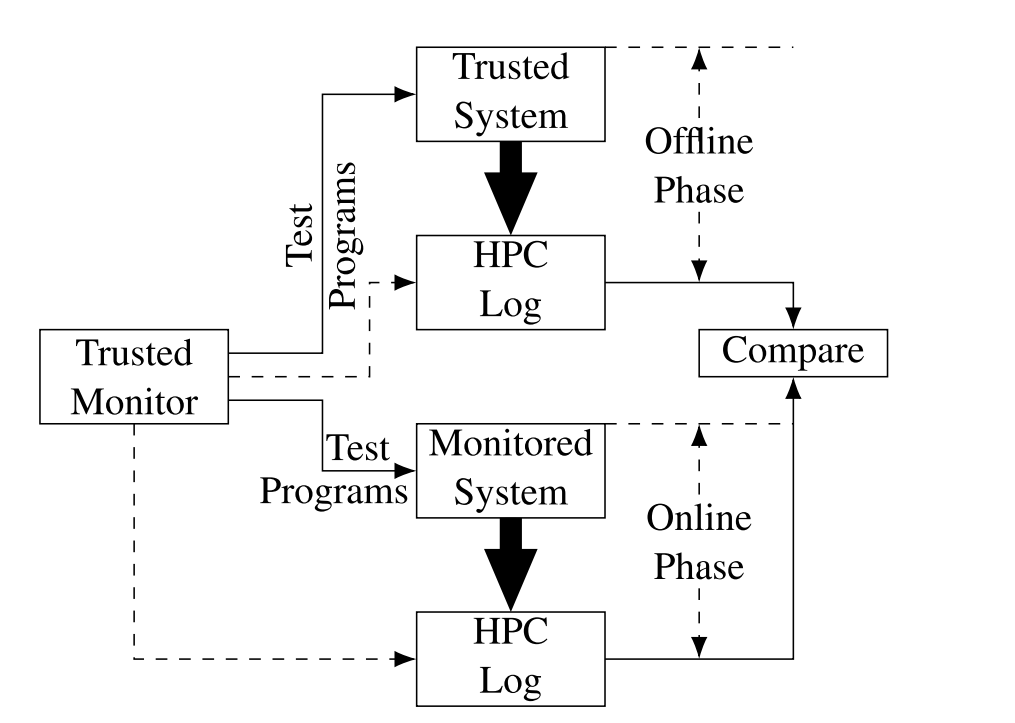
\includegraphics[width=150pt, height=100pt]{contents/images/theoretical_1.png}
    \caption{Taken from \cite{theoretical}: An Overview of HPC-based malware detection}
    \label{fig:theoretical_1}
\end{figure}

The online phase of the HPC-based malware detection system can, either, be used for profiling. The online phase, is used to collect HPC readings from the system and compared to the "golden" readings, if an inconsistency is found it's reported.

The point of this paper is to build a framework to analyze the security guarantees offered by the HPC-based malware detection and create a mathematical representation of the probability of malware detection. The entirety of the paper sits on the usage of a control-flow graph (CFG) as the representation of a program. A CFG is a directed graph in which the nodes represent the basic blocks of the program and the edges represent the control flow paths between them \cite{theoretical}. In this study, the CHStone benchmark is used, since they are data-intensive and lack branching instructions, which should complicate malware detection via HPCs, specifically \textit{sha, motion, mips, jpeg, gsm, blowfish, adpcm} are used. For this experiment only four HPCs are considered:

\begin{itemize}
    \item \textbf{INSTN:} \# of instructions
    \item \textbf{BRNCH:} \# of branches
    \item \textbf{BRNCHT:} \# of branches taken
    \item \textbf{INTGR:} \# of integer instructions
\end{itemize}

Below is the table that breaks down the various details regarding the benchmarks:
\begin{figure}[h]
    \centering
    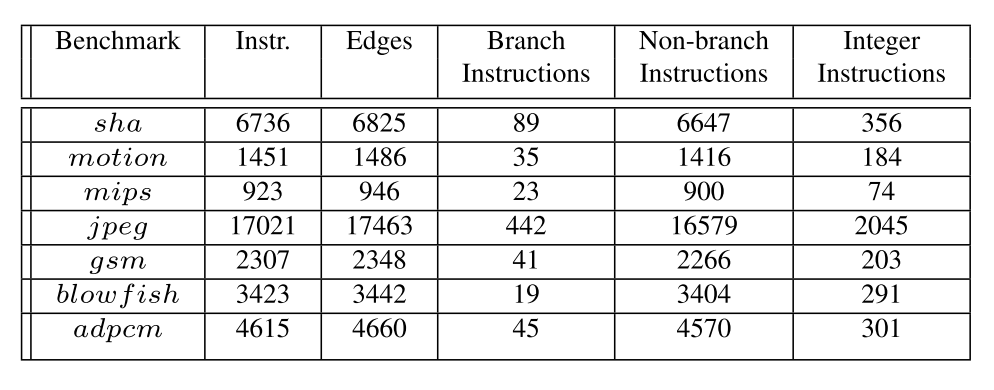
\includegraphics[width=200pt, height=100pt]{contents/images/theoretical_2.png}
    \caption{Taken from \cite{theoretical}}
    \label{fig:theoretical_2}
\end{figure}

The next step is to preform a static and dynamic analysis for each HPC. To handle this two new concepts are introduced \cite{theoretical}:
\begin{enumerate}

    \item \emph{Matching Pairs:} Paths in a CFG whose HPC readings match in all sampling intervals. The probability of detecting a matching pair is given below: \\ 
    \[P_m = \frac{m}{M} = \frac{m}{{n \choose 2}}\]
    where \(M\) is the number of possible matching pairs, \(m\) is the number of matching pairs, and \(n\) is the total number of paths.

    \item \emph{Maximum Matches:} The maximum probability that a path will match any other paths for a specific \(C\), number of cycles and \(s\), HPC sampling interval. The probvability of maximum matches is given by \(m\), the maximum matches and \(n\), the total number of paths in the CFG:
    \[P = \frac{m}{n - 1}\]

\end{enumerate}

The main takeaway from this study was that as sampling rate is increased the probability of matching pairs increases, as well as, the probability of maximum matches. However, the probability decreases as more HPCs are taken in to consideration, with 2 HPCs in consideration resulting in the highest probability of both maximum matches and matching pairs.


\end{document}